\documentclass{article}
\usepackage{graphicx} % Required for inserting images
\usepackage[a4paper, margin=1.2in]{geometry}
\usepackage{amsmath}
\usepackage{amssymb}

%\usepackage{listings}

\usepackage{hyperref}

\title{Exploring Aliasing and the Sampling Theorem} %\\\large\textit{Approximation Part 2 Assignment}}
\author{Margherita Tonon}
\date{April 2025}

\begin{document}

\maketitle

\section{Introduction}
%introduction sentence, context, motivation

\section{Background}
In signal processing, two types of signals exist: analog signals and digital signals. %check that this is true/rephrase
An analog signal refers to a signal that varies continuously over time. 
The complexity of analog signal processing, their susceptibility to noise and signal degradation over time, as well as their limited reproductibility and scalability makes them inconvenient to work with in practice. 
Therefore, digital signals are used -- signals that vary discretely over time and can take only a finite number of distinct values.
%mention advantages of digital signals?

Sampling refers to the process of converting an analog signal into a digital signal. If we let $x(t)$ be a continuous time signal, the sampled signal $x[n]$ is defined as
\begin{center}
    \begin{math}
        x[n] = x(nT_s)
    \end{math}  
\end{center}
where $n$ represents discrete time sampling points and $T_s$ represents the sampling period, such that the sampling frequency $f_s = \frac{1}{T_s}$.

Sampling can also be represented as 
\begin{center}
    \begin{math}
        x_s(t) = x(t) \sum_{-\infty}^{\infty} \delta (t-nT_s)
    \end{math}  
\end{center}
where $x_s(t)$ is the sampled points, and $\delta$ is the dirac delta distribution, taking value 1 if $t=nT_s$, and 0 otherwise.
Therefore, it is clear that when $t=nT_s$, $x_s(t) = x(t)$; otherwise, $x_s(t) = 0$. 

In practice, sampling allows us to discretize a continuous input, facilitating the handling of signals. After sampling is done, it is natural that the signal must be reconstructed in order to recover the original (time continuous) signal.
However, recovery is not always perfect -- the Shannon-Nyquist condition must be met.
%something along the lines of: the key issue is what must the sampling frequency be in order for a signal to be perfectly reconstructed and recovered?

The Shannon-Nyquist theorem states that a signal can be perfectly reconstructed if the sampling frequency is greater than two times the maximum frequency $B$ of the continuous signal:
\begin{center}
    \begin{math}
        f_s > 2B
    \end{math}  
\end{center}
For example, if we consider a sine wave with frequency 5 Hertz, $\sin(2\pi \cdot 5 \cdot t)$, once sampled it can be perfectly reconstructed if the sampling frequency is greater than 10.
%TODO: need to check what the relationship between B and the max continuous frequency is

%do i explain quantization here?

In the time domain, a sampled signal looks like discrete spikes (Figure 1). 
\begin{figure}
    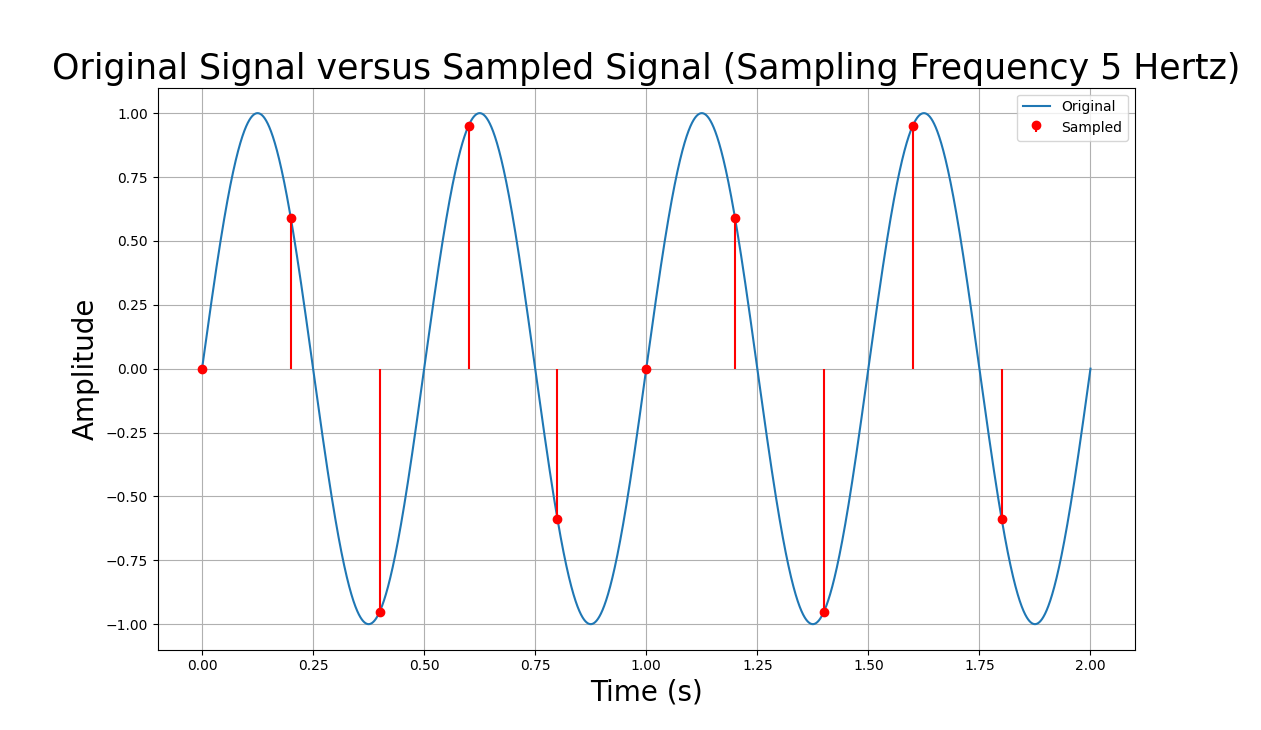
\includegraphics[width=\linewidth]{ogvssampled_BIG.png}
    \caption{Representation of sampling of $\sin(4\pi t)$ in the time domain, sampled at a frequency of 5 Hertz}
    \label{fig:grid}

\end{figure}
The Fourier Transform allows us to transition from the time domain into the frequency domain, and therefore, to visualize what sampling looks like in the frequency domain, we make use of the Inverse Convolution Theorem.

The Inverse Convolution Theorem states that if we have two functions $x(t)$ and $h(t)$ whose Fourier Transforms $\mathcal{F}(x(t))$ and $\mathcal{F}(h(t))$ are absolutely integrable in the frequency domain,
then 
\begin{center}
    \begin{math}
        \mathcal{F}^{-1} \left(X(f) * H(f) \right) = x(t) \cdot h(t)
    \end{math}  
\end{center}
where $*$ is the operation which represents a convolution. %i dont know if i like the syntax "is the operation which represents a convolution" --> is the convolution operator (but maybe wrong)?
Consequently,
%but check if there are additional conditions for this --> I think that this has somethign to do with real numbers
\begin{center}
    \begin{math}
        X(f) * H(f) = \mathcal{F}\left(x(t) \cdot h(t)\right)
    \end{math}  
\end{center}
%if $x(t)$ and $h(t)$ are two absolutely integrable functions in $\mathcal{L}^1(\mathbb{R})$, and if their Fourier transforms $\mathcal{F}(x(t))$ and $\mathcal{F}(h(t))$ exist and are well defined,

Therefore, because we can express sampling as $x_s(t) = x(t) \cdot \sum_{-\infty}^{\infty} \delta (t-nT_s)$ in the time domain, the Inverse Convolution Theorem tells us that %i dont know if here its convolution thm or inverse convolution thm
\begin{center}
    \begin{math}
        \mathcal{F}\left(x(t) \cdot \sum_{-\infty}^{\infty} \delta (t-nT_s)\right) = \mathcal{F}(x(t)) * \mathcal{F}\left( \sum_{-\infty}^{\infty} \delta (t-nT_s) \right)
    \end{math}  
\end{center}

To visualize sampling in the frequency domain we must therefore convolve the Fourier Transform of the input signal with the Fourier Transform of $\sum_{-\infty}^{\infty} \delta (t-nT_s)$, known as the Dirac comb. %not sure this is true
Using properties of the Fourier Transform, Dirac Delta distribution, \_\_\_, %that weird theorem that u can exchange the sum w the integral
and the Poisson summation formula, 
we obtain that 
\begin{center}
    \begin{math}
        \mathcal{F}\left(\sum_{-\infty}^{\infty} \delta (t-nT_s)\right) = \frac{1}{T_s} \sum_{n = -\infty}^{\infty} \delta \left( f - \frac{n}{T_s} \right)
    \end{math}  
\end{center}
% NEED to change the sums so that they look prettier
We therefore have
\begin{center}
    \begin{math}
        \mathcal{F}(x(t)) * \mathcal{F}\left( \sum_{-\infty}^{\infty} \delta (t-nT_s) \right) = X(f) * \frac{1}{T_s} \sum_{n = -\infty}^{\infty} \delta \left( f - \frac{n}{T_s} \right)
    \end{math}  
\end{center}
Convolution of a function with a delta function shifts the function by the shift factor, and therefore %TODO: change the word shift factor here but i dont know to what
\begin{center}
    \begin{math}
        \mathcal{F}(x(t)) * \mathcal{F}\left( \sum_{-\infty}^{\infty} \delta (t-nT_s) \right) = \frac{1}{T_s} X\left(f - \frac{n}{T_s} \right)
    \end{math}  
\end{center}
We can consequently observe how the representation of a sampled signal in the frequency domain is simply the Fourier Transform of the signal, duplicated and shifted to multiples of the sampling frequency. %CHECK THAT THIS IS TRUE

To recover the original signal from the sampled signal, we apply an ideal band pass filter,
\begin{center}
    \begin{math}
        H(f) = %insert the piecewise function of the band pass filter
    \end{math}  
\end{center}

%1 \; \text{if} \; f_l < f < f_h
%0 \; \text{otherwise}

which selects the frequencies between $f_l$ and $f_h$ Hertz. %idk if the frequencies are selected or what is selected --> review
We then perform an inverse Fourier Transform on the signal and we will have recovered the original signal. %check that this is true
%ALSO give a better description of the filtering

Nonetheless, the frequency domain representation of the sampled signal highlights the need for the Shannon-Nyquist theorem. %maybe not "need" but like utility/usefulness or something
When our sampling frequency is ``large enough'', the process of copying and shifting the frequencies occurs at larger intervals, meaning the copied frequencies are more spread out. It is therefore possible to apply an ideal filter to recover the original frequencies. %frequencies or frequency?
However, if the sampling frequency decreases, the interval between frequencies is not as large and they may overlap. It is therefore no longer possible to apply an ideal filter to recover the original frequencies, as the original signal and the duplicated frequencies overlap.
This is known as aliasing: the act of different frequency components becoming indistinguishable in the sampled signal due to overlapping spectra. %maybe use a diff definition cause this is rly similar to the one on the slides
As long as we set $f_s > 2B$, however, the signal is able to be perfectly recovered. 

%maybe give an example of aliasing happening, like the one we saw in class?

%some context into the problem, theory
%overview of what sampling is, why its used!! important to say why sampling
%what happens when we sample?
%the problem of reconstruction and the need for sufficiently high sampling frequencies

\section{Implementation}
%TODO: insert code snippets and change the function names to actual code block writing
%explanation of code
%the theory behind the sinc function bc thats what we implement when we have been talking about ideal band pass filter the entire time
%here dont put all of the different frequencies because we do that in the discussion
To implement the process of sampling in Python, I begin by defining a functionn \verb|generate_signal| which generates a sine wave (a continuous-time signal) of desired frequency.
%\begin{lstlisting}[language = Python]
\begin{verbatim}
    def generate_signal(t_end, frequency, plot = False):
        """
        Generates a sine wave from t = 0 to t=t_end with frequency defined by the frequency parameter.
        If plot = True, plots the generated sine wave.
        Returns the time array t and the x(t) sinusoid.
        """
        t = np.linspace(0, t_end, 10000)
        x = np.sin(2 * np.pi * frequency * t)
        if plot == True:
            plt.plot(t, x)
            plt.title(f"Continuous Time Signal - Sine Wave With Frequency {frequency} Hertz")
            plt.xlabel("Time")
            plt.ylabel("Amplitude")
            plt.grid(True)
            plt.show()
        return t, x
\end{verbatim}
%\end{lstlisting}
%insert code block here
Here, I simply create a time array with 10000 elements, and then apply the sine function with the given frequency to the 10000 time values. 
Users can set the ``plot'' parameter to ``True'' if they wish a plot of the original continuous-time signal to be displayed.

Next, I define the ``sample\_signal'' function, which samples the continuous signal at a specified sampling frequency.
Users can set ``plot\_one'' to ``True'' if they wish to visualize the original signal together with the sampled points, and ``plot\_two'' to True if they wish to just visualize the sampled points.
%code block 
%NEED TO EXPLAIN WHAT IS HAPPENING IN THIS CODE BLOCK

Thirdly, I create the ``sampled\_fourier\_transform'' function, which takes as inputs the sampled amplitudes and the sampling frequency, and performs the Fast Fourier Transform of the sampled amplitudes using the ``scipy'' module. %something that u used scipy
Users can again set the plot parameter to True if they wish to observe the frequencies of the sampled signal in the frequency domain. %something abt this but u have to fix it in the code
%code block

Finally, I define the ``reconstruction'' function, which 

The sinc function, defined as $\text{sinc}(x) = \frac{\sin(\pi x)}{\pi x}$, is utilized as it is the time domain representation of the ideal band pass filter.
%in one of the summary sheets you have more about this --> say why u are using it like that? and no convolution or something?
The sinc function is obtained by taking the inverse Fourier Transform of the ideal band pass filter:
\begin{center}
    \begin{math}
        h(t) = \int_{-\infty}^{\infty} H(f) e^{2\pi i ft} df
    \end{math}  
\end{center}
$H(f)$ is even and real and therefore $e^{2\pi i ft}$ = $\cos(2\pi ft) + i \sin(2\pi ft)$ = $\cos(2\pi ft)$ as the imaginary part is 0.  
\begin{center}
    \begin{math}
        h(t) = \int_{-\infty}^{\infty} H(f) \cos(2\pi ft) df
    \end{math}  
\end{center}
Evaluating this integral,
\begin{center}
    \begin{math}
        h(t) = \frac{1}{\pi t} \left[ \sin(2\pi f_h t) - \sin(2\pi f_l t) \right]
    \end{math}  
\end{center}
This is the difference of two sinc-like functions. 
%TODO: understand the link between the difference of two sinc like functions and the following sentence that we can just recover the signal like this:
The signal $x(t)$ can therefore be recovered in the following way:
\begin{center}
    \begin{math}
        x(t) = \sum_{-\infty}^{\infty} x(nT) \text{sinc}\left( \frac{t}{T} - n \right)
    \end{math}  
\end{center}
which is the approach implemented in the ``reconstruction'' function. 

\section{Discussion}
%results of code
%different initial frequencies, different sampling frequencies based on shannon nyquist thm

\section{Conclusion}
%maybe link to why this is important if this sine wave wasnt just this arbitrary sine wave but rather an actual signal that needed to be transmitted/used

\begin{thebibliography}{9} %TODO turn to MLA
    \bibitem{1} https://realpython.com/python-scipy-fft/
\end{thebibliography}

\section{Appendix}
\begin{enumerate}
    \item Access the GitHub repository with all code \href{https://github.com/margheritatonon/approximation-II-assignment}{here}.
\end{enumerate}


\end{document}
